\chapter{Sailboat regulation}


The original algorithms which were used in order to regulate a sail-boat is given here
\cite{jaulin2015robotique}.

For all those algorithms, we decide to chose one specific situation and we express the regulator in order to generate a potential adapted to the situation. For example, the following algorithm is used for the line regulation of the sail-boat \ref{alg:MYALG_line}.

\begin{algorithm}[H]
  \caption{Sail-boat regulator , line }
  \label{alg:MYALG_line}
  \textbf{Inputs}% Inputs section
  \begin{algorithmic}[1]
    \STATE $m$ position of the sailboat
    \STATE $\theta$ heading of the sail-boat
    \STATE $\psi$ wind direction
    \STATE $a,b$ point of the line
    \STATE $q$ hysteresis
  \end{algorithmic}
  \bigskip

  \textbf{Output}% Output section
  \begin{algorithmic}[1]
    \STATE $\delta_r$ ruder angle
    \STATE $\delta_s$ sail angle
    \STATE $q$ hysteresis
  \end{algorithmic}
  \bigskip
  
  \textbf{Initialization}% Initialization section
  \begin{algorithmic}[1]
   	\STATE $q\gets 1$
  \end{algorithmic}
  
  
  \textbf{Algorithm}
  \begin{algorithmic}[1]
  	\STATE $e = det(\frac{b-a}{||b-a||},m-a)$
  	
  		\IF{$|e|>\frac{r}{2}$}
  			\STATE q = sign(e)
  		\ENDIF
  		
  		\STATE $\varphi = atan2(b-a)$
  		\STATE $\theta^* = \varphi - \frac{2\gamma_{\infty}}{\pi} . atan(\frac{e}{r})$
	 	\IF{ cos($\psi$-$\theta^*$)+cos($\zeta$) < 0 or ($|e|<r$ and cos($\psi$-$\varphi$)  + cos($\zeta$))}
     	  	\STATE $\theta_p$ = $\pi$ + $\psi$ - q . $\zeta$
     	
		\ELSE
			\STATE $\theta_p$ = $\theta^*$
	 	\ENDIF
	 	
  \STATE $\delta_r$ = $\frac{\delta_s^{max}}{\pi} . atan(tan(\frac{\theta-\theta_p}{2}))$
  
  \STATE $\delta_s$ = $\delta_s^{max} . \frac{cos(\psi-\theta_p)+1}{2}$
	
  \end{algorithmic}
\end{algorithm}

In the end, we generate a field potential as below which allow the sail-boat to follow the line.

\begin{figure}[H]
\centering
    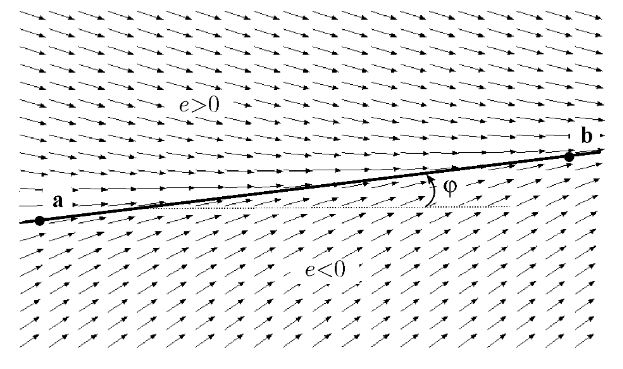
\includegraphics[scale=0.5,angle=0]{Images/FieldVector.png}
    \caption{Field potential generated by this regulator.}
    \label{fig:FieldVector}
\end{figure}


\chapter{Generation of field potential}


Nevertheless, we wanted to realize a new version of this algorithm which would allow us to get the value of the ruder angle and the sail angle by only providing the heading wanted, the real heading and the wind direction. 




\chapter{update of the algorithm}

The following algorithm is the result of our work \ref{alg:MYALG}.


\begin{algorithm}[H]
  \caption{Sail-boat regulator V1 }
  \label{alg:MYALG}
  \textbf{Inputs}% Inputs section
  \begin{algorithmic}[1]
    \STATE $\theta^*$ heading wanted
    \STATE $\theta$ heading of the sail-boat
    \STATE $\psi$ wind direction
    \STATE q hysteresis
  \end{algorithmic}
  \bigskip

  \textbf{Output}% Output section
  \begin{algorithmic}[1]
    \STATE $\delta_r$ ruder angle
    \STATE $\delta_s$ sail angle
    \STATE q hysteresis
  \end{algorithmic}
  \bigskip
  
  \textbf{Initialization}% Initialization section
  \begin{algorithmic}[1]
   	\STATE $q\gets 1$
  \end{algorithmic}
  
  
  \textbf{Algorithm}
  \begin{algorithmic}[1]
	 	\IF{ cos($\psi$-$\theta^*$)+cos($\zeta$) < 0}
	 		\STATE q = sign(sin($\psi-\theta^*$))
     	  	\STATE $\theta_p$ = $\pi$ + $\psi$ - q . $\zeta$
     	
		\ELSE
			\STATE $\theta_p$ = $\theta^*$
	 	\ENDIF
	 	
  \STATE $\delta_r$ = $\frac{\delta_s^{max}}{\pi} . atan(tan(\frac{\theta-\theta_p}{2}))$
  
  \STATE $\delta_s$ = $\delta_s^{max} . \frac{cos(\psi-\theta_p)+1}{2}$
	
  \end{algorithmic}
\end{algorithm}




